%!TEX root = ./template-skripsi.tex
%-------------------------------------------------------------------------------
%                            	BAB III
%               		    METODE PENELITIAN
%-------------------------------------------------------------------------------

\chapter{METODE PENELITIAN}

\section{Deskripsi Sistem}
    Sistem bertujuan untuk melakukan penghitungan panjang serta berat objek ikan yang menggunakan
metode \emph{Harris-corners} dan \emph{Gausian Laplace}. Penelitian berfokus dalam menghasilkan berupa
data hasil panjang dan berat objek ikan. Dataset citra ikan diambil secara langsung menggunakan \emph{Smartphone} pada sebuah
penangkaran ikan. Kemudian bahasa yang akan digunakan dalam membangun sistem adalah Python versi 3.

Tahapan dalam penghitungan panjang dan berat ikan menggunakan \emph{Harris-Corner Detection} adalah Pemrosesan Citra,
\emph{Smoothing Gaussian}, Perhitungan gradien, autokorelasi matriks gradien, \emph{Harris Respons}, melakukan threshold-ing dan \emph{Non-Maximum Suppression}, menentukan koordinat sudut, perhitungan panjang dan lebar, Penghitungan berat,
dan terakhir adalah mengasosiasikan data.

\section{Perancangan Sistem}
    Pada bagian ini akan menbahas tentang proses yang akan dilakukan untuk mengetahui tahapan yang ditempuh
dalam membangun sistem penghitungan berat dan panjang ikan. Tahapan pertama yang dilakukan adalah melakukan \emph{input} gambar
yang akan dibaca sistem, setelah itu citra akan diproses menggunakan \emph{Smoothing gaussian} untuk menggurangi \emph{noise}. Kemudian perhitungan gradien dilakukan bertujuan untuk menghitung setiap perubahan intensitas yang berada di sekitar titik, 
hasil tersebut akan diolah kembali menggunakan autokorelasi matriks gradien, dan dilanjutkan dengan menjalakan \emph{Harris respons}. \emph{Harris respons} bertujuan untuk mengetahui bahwa titik tersebut adalah sebuah sudut, sisi, atau tepi berdasarkan pada hasil respon harris. 
Hasil dari harris akan memasuki tahapan thresholding dan \emph{non-maximum suppression} untuk memilih sudut maximum pada area tertentu. Setelah mendapatkan titik yang merupakan sebuah sisi, titik-titik tersebut akan dipilih. 
Dimana hasil dari pemilihan tersebut akan menjadi cara untuk dapat menghitung panjang, lebar dan berat ikan. Gambaran perancangan sistem yang sederhana bisa dilihat pada gambar \ref*{Alur Penelitian}

\begin{figure}
    \centering
    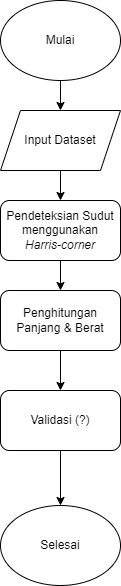
\includegraphics[scale= 0.6]{gambar/Flowchar Penetianv2.png}
    \caption{Alur Penelitian}
    \label{Alur Penelitian}
\end{figure}

\subsection{Pemrosesan Citra}
    Gambar yang akan digunakan berformat .jpg atau .png, dengan latar belakang yang telah dihilangkan dan digantikan dengan warna solid. 
Gambar tersebut akan diubah dari format RGB menjadi citra \emph{grayscale}. Perubahan ini diperlukan untuk mempermudah proses pendeteksian sudut. 


\subsection{Smoothing Gaussian}
    Metode \emph{Smoothing Gaussian} digunakan untuk mengurangi \emph{noise} pada gambar sebelum melanjutkan ke perhitungan lebih lanjut.
\emph{Noise} adalah gangguan yang muncul dalam gambar digital yang dapat mengaburkan detail atau informasi penting. \emph{noise} dapat disebabkan oleh berbagai faktor, seperti kualitas sensor kamera yang rendah, pencahayaan yang buruk, atau kesalahan dalam proses pemindahan data.
Dalam gambar, \emph{noise} biasanya terlihat sebagai bintik-bintik acak atau intensitas piksel yang tidak diinginkan. Keberadaan \emph{noise} ini dapat menjadi masalah dalam proses pendeteksian sudut, karena \emph{noise} dapat menyebabkan munculnya sudut palsu yang tidak sesuai dengan gambar asli.
    
    Langkah pertama dalam \emph{smoothing Gaussian} adalah membentuk \emph{Gaussian kernel}. Pemilihan ukuran kernel sangat berpengaruh terhadap hasil \emph{smoothing}, khususnya pada tingkat kehalusan gambar dan jumlah \emph{noise} yang berkurang.
Semakin besar kernel yang digunakan, semakin banyak \emph{noise} yang dihilangkan, tetapi hal ini dapat menyebabkan detail gambar ikut terhapus. Sebaliknya, jika kernel yang digunakan berukuran kecil, detail gambar akan lebih terjaga, tetapi \emph{noise} mungkin masih tetap ada.
Setelah menentukan ukuran kernel yang akan digunakan kernel dapat dihitung dengan menggunakan persamaan \eqref{eq:gaussian kernel}.

    Langkah selanjutnya adalah mengaplikasikan kernel pada gambar. Proses ini dilakukan dengan menerapkan kernel secara berulang pada setiap piksel di seluruh gambar.
Namun, sebelum langkah tersebut, gambar perlu di-\emph{padding} terlebih dahulu. \emph{Padding} adalah proses menambahkan piksel pada tepi gambar sebelum pemrosesan dengan kernel atau model dimulai.
Tujuan dari \emph{padding} adalah untuk mempertahankan ukuran gambar setelah diterapkannya operasi tertentu, seperti konvolusi. 
Setelah \emph{padding} diterapkan, konvolusi akan dilakukan dengan menggunakan persamaan \eqref{eq:konvolusi} . 

\subsection{Perhitungan Gradien}
    Gambar yang telah diperhalus akan dilanjutkan dengan menghitung gradient pada setiap \emph{pixel}-nya. Tujuan dari penghitungan gradien adalah untuk mengetahui perubahan intensitas pada setiap piksel, yang pada umumnya akan menujukan tepi atau kontur dalam sebuah gambar.
Penghitungan gradient juga memerlukan kernel untuk dapat bekerja, terdapat banyak kernel yang dapat digunakan untuk menghitung gradient, contohnya kernel sobel. 

    Kernel Sobel digunakan untuk menghitung estimasi gradien dengan memberikan bobot yang lebih besar pada piksel tetangga terdekat di sekitar piksel pusat.
Kernel sobel terdiri dari dua matriks \(3 x 3\), yang bertujuan untuk menghitung gradient pada dua arah yaitu:
 \begin{itemize}
    \item \textbf{Gradien Horizontal} \((G_{x})\): Mengukur perubahan intensitas sepanjang sumbu x.
    \item \textbf{Gradien Vertical} \((G_{y})\): Mengukur perubahan intensitas sepanjang sumbu y.
\end{itemize}
    Berikut adalah kernel yang akan digunakan dalam operator sobel :
\begin{enumerate}
    \item Kernel Sobel Horizontal
    \begin{equation*}
        S_{x} = 
        \begin{bmatrix}
            -1 & 0 & 1 \\
            -2 & 0 & 2 \\
            -1 & 0 & 1
          \end{bmatrix}
    \end{equation*}

    \item  Kernel Sobel Vertical
    \begin{equation*}
        S_{y} = 
        \begin{bmatrix}
            -1 & -2 & -1 \\
            0 & 0 & 0 \\
            1 & 2 & 1
          \end{bmatrix}
    \end{equation*}

\end{enumerate}
Perhitungan gradien juga akan menggunakan rumus \eqref{eq:konvolusi} tetapi gaussian filter akan diganti dengan kernel sobel horizontal (Gx) dan kernel sobel vertical (Gy).
Maka rumusannya akan seperti berikut :
\begin{equation}
    \begin{aligned}
        G_{x} = Sx * I(x)\\ G_{y} = Sy * I(x)
    \end{aligned}
\end{equation}


\subsection{Menghitung Second Moment Matriks}
    Setelah hasil dari perhitungan gradien didapatkan, hasil tersebut akan dibuat menjadi matriks kembali dengan rumus \eqref{SecondMomentMatrix}. Nilai gradien dihitung untuk mendapatkan koefisien matriks autokorelasi. Setelah koefisien didapatkan, koefisien tersebut akan dikonvolusi dengan filter gaussian.
Baru setelah itu hasil dari konvolusi digunakan untuk membentuk matriks \(M\) yang akan digunakan untuk perhitungan selanjutnya. Bentuk dari matriks \(M\) sebagai berikut :

\begin{equation*}
    \begin{aligned}
        \Sigma I_{x} = g(\sigma) * G_{x}^2 \\
        \Sigma I_{x}I_{y} = g(\sigma) * G_{x} * G_{y} \\
        \Sigma I_{y} = g(\sigma) * G_{y}^2
    \end{aligned}
\end{equation*}

\begin{equation}
    M = 
    \begin{bmatrix}
        \Sigma I_{x} & \Sigma I_{x}I_{y} \\
        \Sigma I_{x}I_{y} & \Sigma I_{y}
    \end{bmatrix} 
\end{equation}

\subsection{Harris Respon}
    Matriks \(M\) digunakan untuk menghitung respon harris, menggunakan rumus harris yaitu:
\begin{equation}
    R(x,y) = Det(M) - k * (trace(M))^2
\end{equation}
Dimana \(Det(M)\) :
\begin{equation*}
    Det(M) = \Sigma I_{x} * \Sigma I_{y} - \Sigma I_{x}I_{y}^2
\end{equation*}
Dan \(trace(M)\) 
\begin{equation*}
    trace(M) = \Sigma I_{x} + \Sigma I_{y}
\end{equation*}

    Penggunaan harris respon bertujuan untuk menandai bahwa piksel tersebut adalah sudut atau tidak.


\subsection{Thresholding dan \emph{Non-Maximum suppression}}
    Setelah nilai harris didapatkan tahapan langkah selanjutnya adalah melakukan Thresholding.
Thresholding adalah cara untuk memilih hasil deteksi dengan cara menetapkan nilai ambang batas.
Jika nilai harris melebihi dari ambang batas, maka piksel tersebut akan dianggap sebagai potensial sudut kuat, Sebaliknya jika nilai harris lebih kecil maka piksel tersebut akan diabaikan.
Tujuannya supaya mengurangi piksel yang perlu menjadi diproses lebih lanjut. 
\begin{equation}
    Corner(x,y) = 
    \begin{cases}  
        1 & \text{jika } R(x,y) > T \\ 
        0 & \text{jika } R(x,y) <= T
    \end{cases}
\end{equation}

    Setelah melewatin Thresholding, setiap piksel yang telah lolos akan diperiksa kembali dengan \emph{Non-Maximum Suppression} atau NMS.
NMS bertujuan untuk mengelolah kembali piksel yang saling berdekatan satu sama lain. NMS akan memilih piksel pada \emph{range} tertentu, piksel dengan nilai \(R\) terbesar akan terpilih sebagai puncak lokan dan dipertahankan sebagai sudut, dan yang lainnya akan diabaikan.
\begin{equation*}
    NMS(x,y) =
    \begin{cases}
        1 & \text{jika } R(x,y) = MaxLocal R(i,j) \\
        0 & \text{lainnya }
    \end{cases}
\end{equation*}
Dimana \emph{MaxLocal} \(R(i,j)\) adalah nilai maksimum yang berada disekitar piksel \((x,y)\).

\subsection{Memilih Piksel}
    Setelah sudut telah melalui Thresholding dan NMS, sudut-sudut tersebut akan dipilih berdasarkan kriteria yang telah ditentukan.
\begin{enumerate}
    \item Sudut berada pada bagian ekor.
    \item Sudut berada pada bagian mulut.
    \item Sudut berada pada bagian sirip atas.
    \item Sudut berada pada bagian bawah atau perut.
\end{enumerate}

Keempat kriteria tersebut dibutuhkan untuk mempermudah dalam penghitungan panjang dan lebar.


\subsection{Menghitung Panjang dan Berat}
    Rumus untuk menghitung panjang dan lebar dengan menggunakan koordinat yang telah dipilih adalah sebagai berikut :
\begin{equation}
    d = \sqrt{(x_2 - x_1)^2 + (y_2 - y_1)^2}
\end{equation}    

    Untuk menghitung panjang dan lebar asli sebuah benda dalam gambar dibutuhkan dua hal, yaitu skala dan panjang benda pada gambar.
Skala dapat dicari dengan dua cara yaitu menggunakan benda referensi, atau dengan menggunakan resolusi pada gambar tersebut.
    
    Kedua cara tersebut memilik kelebihan dan kekurang masing-masing, contohnya menggunakan benda referensi.
 Metode ini memerlukan benda lain dalam gambar dan mengetahui panjang dari benda lain tersebut, jika tidak ada benda lain pada gambar diperlukan pengambilan gambar pada jarak yang sama dengan benda yang ingin dicari panjangnya.
 Kelebihan dari metode ini adalah akurasi yang tinggi, metode selanjutnya juga sama menggunakan resolusi gambar dapat mempermudah penghitungan, namun akurasi dari penghitungan panjang akan berkurang.
\begin{equation*}
    Skala = \frac{Ukurang Nyata}{Ukuran gambar}
\end{equation*}

\begin{equation}
    Jarak Nyata = Jarak gambar * Skala
\end{equation}

    Setelah diketahui panjang dan lebar, langkah berikutnya adalah menghitung berat. Penghitungan berat pada gambar akan dilakukan dengan menggunakan interpolasi dengan data yang telah diambil. Menggunakan rumus sebagai berikut:
\begin{equation}
    Wn = Wx + (Ln - Lx / Ly - Lx) * (Wy - Wx)
\end{equation}
Dimana 
\begin{itemize} 
    \item Wn berat yang dicari.
    \item Wx berat sebelum.
    \item Wy berat sesudah.
    \item Ln Luas dari berat yang dicari.
    \item Lx Luas dari berat sebelum.
    \item Ly Luas dari berat sesudah.
\end{itemize}
    Jika diatas akan dilakukan kembali jika lebar dari ikan juga berbeda.

